% первая часть

\section{Предметная область}

\url{https://www.genebm.com/drone-bytes/software-design/middlewares-ros-fprime} часть обоснования выбора рос

\subsection{Математическая модель квадрокоптера}
Рассмотрим квадрокоптер с известными физическими параметрами, движением которого можно управлять, изменяя скорости вращения винтов. Для формального описания динамики движения квадрокоптера как твердого объекта в трёхмерном пространстве необходимо ввести в рассмотрение две системы координат (СК):
1. Неподвижную систему координат (НСК), в качестве которой выступает нормальная земная система координат с заданными перпендикулярными друг другу координатными осями \(O_{g}X_{g}\), \(O_{g}Y_{g}\), и \(O_{g}Z_{g}\), причем ось \(O_{g}Z_{g}\) направлена противоположно вектору силы тяжести.
2. Связанную с квадрокоптером систему координат (ССК), центр которой размещен в центре масс аппарата, а оси OX, OY, и OZ параллельны и сонаправлены с осями неподвижной системы. Угловое положение аппарата зададим тремя углами Эйлера: углами крена \(\phi\), тангажа \(\theta\) и рыскания \(\psi]\), определяющими вращение вокруг осей OX, OY, и OZ соответственно. Основываясь на ранее рассмотренных системах координат можно утверждать о том, что квадрокоптер имеет шесть степеней свободы, а именно три линейных координаты [x; y; z ] и три угловых \([\theta, \phi, \psi]\). В качестве управляющих каналов выступают скорости вращения роторов (рис. 1), которые создают динамику движения БПЛА в пространстве. Согласно (1–3), возникающие в результате подачи управляющих воздействий силы и моменты пропорциональны квадрату угловых скоростей винтов \(\Omega^2\) . Поэтому, для достижения желаемого режима работы БПЛА, необходимо связать совокупность управляющих воздействий со степенями свободы БПЛА, через уравнения связи, которые определяют основные режимы движения квадрокоптера в пространстве.

% ~\ref{fig:ris1}
\begin{figure}[H]
	\centering
	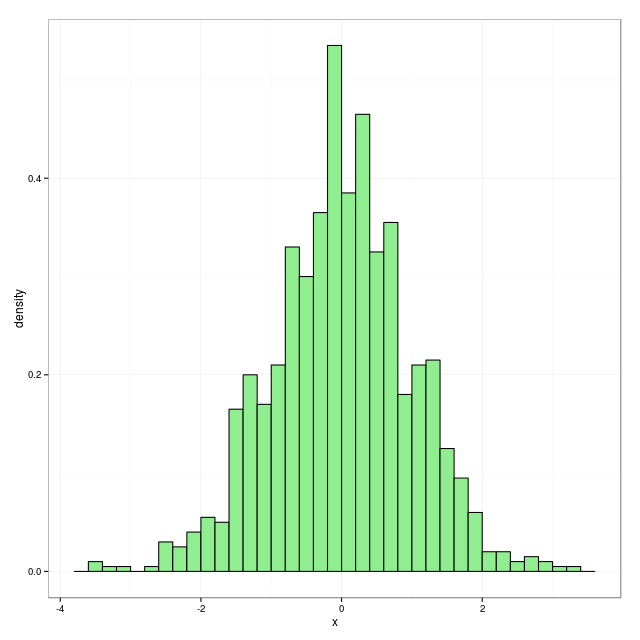
\includegraphics[width=0.5\linewidth]{pics/ris1}
	\caption{Связанная система координат квадрокоптера
	}
	\label{fig:ris1} % эта метка позволяет ссылаться на рисунок в тексте
\end{figure}
В качестве первого режима БПЛА \(U_{1}\) рассмотрим движение вдоль оси OZ, принадлежащей ССК. Данное движение обеспечивается одновременным увеличением скоростей винтов на одинаковое значение угловой скорости \(\Delta a\). Полученное при этом движение (рис. ~\ref{fig:ris1}) характеризуется взлетом или посадкой квадрокоптера (при нулевых значениях тангажа и крена) и описывается следующим выражением:
\begin{equation}
U_{1}=b(\Omega_{1}^2+\Omega_{2}^2+\Omega_{3}^2+\Omega_{4}^2)
\end{equation}
где b – аэродинамическая составляющая тяги винта.
В качестве второго режима движения БПЛА \(U_{2}\) необходимо взять поворот вокруг оси OX, принадлежащей ССК. Данное движение достигается путем увеличения/уменьшения на величину \(\Delta a\) значения \(\Omega_{4}\) левого винта и уменьшением/увеличением на величину \(\Delta b\) значения \(\Omega_{1}\)
правого. Полученное при этом движение характеризуется изменением угла крена \(\phi\) (рис. ~\ref{fig:ris2}) и описывается следующим выражением:
\begin{equation}
U_{2}=lb(-\Omega_{2}^2-\Omega_{4}^2)
\end{equation}
где l – расстояние между центром квадрокоптера и центром винта.
% ~\ref{fig:ris2}
\begin{figure}[H]
	\centering
	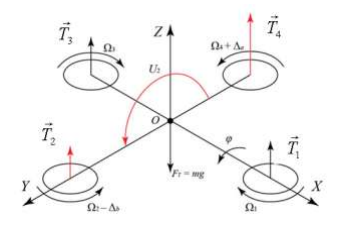
\includegraphics[width=0.5\linewidth]{pics/ris2}
	\caption{Вращение квадрокоптера вокруг оси OX
	}
	\label{fig:ris2} % эта метка позволяет ссылаться на рисунок в тексте
\end{figure}
В качестве третьего режима движения \(U_{3}\) необходимо взять поворот БПЛА вокруг оси OY , принадлежащей ССК. Данное движение достигается путем уменьшения/увеличения на величину \(\Delta a\) значения \(\Omega_{1}\) фронтального винта и увеличения/уменьшения на величину \(\Delta b\) значения \(\Omega_{3}\) заднего. Полученное при этом движение характеризуется изменением угла тангажа \(\theta\) (рис. ~\ref{fig:ris2}, а) и описывается следующим выражением:
\begin{equation}
U_{3}=lb(-\Omega_{1}^2-\Omega_{3}^2)
\end{equation}
% ~\ref{fig:ris3}
\begin{figure}[H]
	\centering
	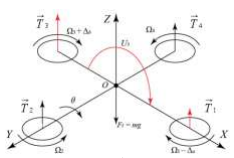
\includegraphics[width=0.5\linewidth]{pics/ris3}
	\caption{Вращение вокруг оси OY
	}
	\label{fig:ris3} % эта метка позволяет ссылаться на рисунок в тексте
\end{figure}
% ~\ref{fig:ris4}
\begin{figure}[H]
	\centering
	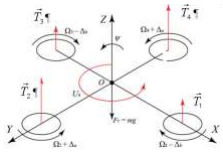
\includegraphics[width=0.5\linewidth]{pics/ris4}
	\caption{Вращение вокруг оси OZ
	}
	\label{fig:ris4} % эта метка позволяет ссылаться на рисунок в тексте
\end{figure}
Рис. 3 – Режимы движения квадрокоптера
 % переделать на две картинки рядом
В качестве последнего, четвертого, режима движения \(U_{4}\) необходимо взять поворот БПЛА вокруг оси OZ , принадлежащей ССК. Данное движение достигается путем одновременного увеличения/уменьшения на величину \(\Delta a\) значений \(\Omega_{4}\) левого и \(\Omega_{2}\) правого винтов, а также одновременного уменьшения/увеличения на величину \(\Delta b\) значений \(\Omega_{1}\) фронтального и \(\Omega_{3}\) заднего винтов. Благодаря вращению роторов в диагонально противоположных направлениях, полученное движение характеризуется изменением угла рыскания \(\psi\) (рис. 3, б) и описывается следующим выражением:
\begin{equation}
U_{4}=d(-\Omega_{1}^2+\Omega_{2}^2-\Omega_{3}^2+\Omega_{4}^2)
\end{equation}
где d – аэродинамическая составляющая коэффициента сопротивления среды.
Введенное, с учетом (1) – (4), множество U, характеризующее режимы
движения квадрокоптера можно записать следующим образом:
\begin{numcases}{U=}
U_{1}=b(\Omega_{1}^2+\Omega_{2}^2+\Omega_{3}^2+\Omega_{4}^2)\\
U_{2}=lb(-\Omega_{2}^2-\Omega_{4}^2)\\
U_{3}=lb(-\Omega_{1}^2-\Omega_{3}^2)\\
U_{4}=d(-\Omega_{1}^2+\Omega_{2}^2-\Omega_{3}^2+\Omega_{4}^2)
\end{numcases}
Множество U определяет связь между системой исполнительных приводов и платформой БПЛА. Поэтому, при дальнейшем рассмотрении математической модели динамики движения квадрокоптера, режимы движения (1) –
(4) будут использоваться как задающие воздействия для платформы БПЛА.

\subsection{Физическая модель квадрокоптера}

Квадрокоптер состоит из:

--- полетного контроллера,

--- 4 регуляторов оборотов,

--- 4 моторов,

--- рамы,

--- камеры,

--- видеопередатчика,

--- видеоантенны,

--- радиоприемника,

--- другой периферии

 % ~\ref{fig:drone}
 \begin{figure}[H]
 	\centering
 	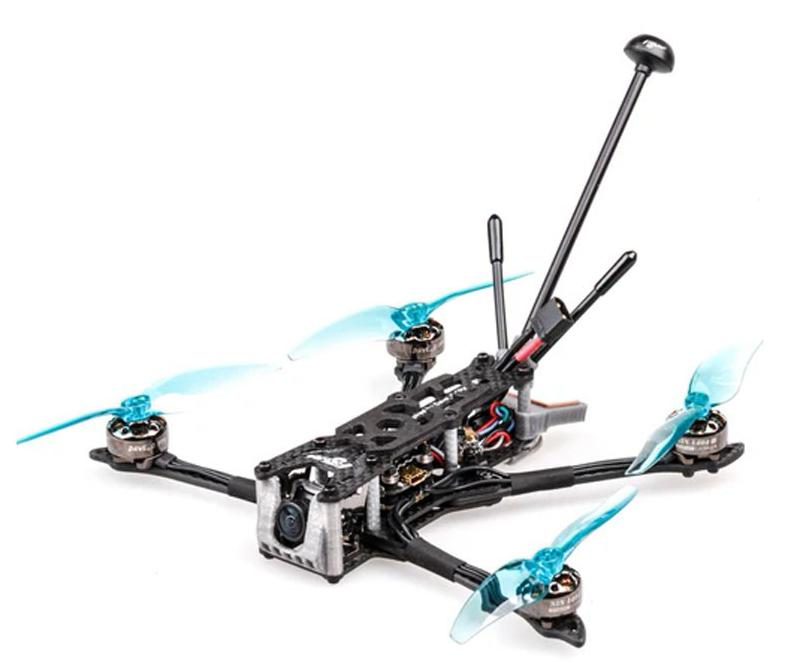
\includegraphics[width=0.5\linewidth]{pics/drone}
 	\caption{Пример квадрокоптера
 	}
 	\label{fig:drone} % эта метка позволяет ссылаться на рисунок в тексте
 \end{figure}
Рама - несущий компонент, на котором располагается вся электроника квадрокоптера. В большинстве случаев представляет собой крестообразную конструкцию. Рама должна быть жесткой, чтобы не создавать осцилляции для ПИД регулятора, и в то же время легкой. На данный момент лучшим материалом для рам квадрокоптеров является карбон.

Видеосистема состоит из трех основных компонентов: камера, видеопередатчик и передающая антенна. Видеопередатчик на частоте 5.8ГГц и указанной мощности передает изображение с камеры.

Моторы - основные компоненты беспилотных летательных аппаратов. В зависимости от их количества добавляется числовая приставка к слову коптер. Для современных БПЛА используются бесколлекторные моторы. Основными их характеристиками являются скорость, тяговооруженность, количество оборотов на вольт. В зависимости от перечисленных характеристик, веса летательного аппарата и выбранного аккумулятора подбираются пропеллеры.

Диаметр пропеллера и количество лопастей определяют статическую тягу квадрокоптера. Шаг пропеллера определяет скорость потока воздуха.

Количество оборотов в каждый момент времени определяет регулятор оборотов. Он представляет собой электрическую цепь, передающую энергию от батареи к двигателю, преобразуя постоянный ток источника питания в переменный ток, который нужен мотору. Количество оборотов мотора определяет полетный контроллер.

Для питания квадрокоптера используются литий-полимерные и литий-ионные аккумуляторы. В зависимости от задач и размеров подбирается количество ячеек аккумулятора, емкость и токоотдача.

Полетный контроллер -- система реального времени, которая интерпретирует входящие данных от приемника и бортовых датчиков, на основе которых рассчитывает и передает ШИМ на регуляторы оборотов и тем самым производится регулировка скорости моторов. Все алгоритмы работы полетного контроллера содержатся в прошивке -- программном обеспечении, которое выбирается в зависимости от схемы полетного контроллера и поставленных задач.

Для осуществления управления квадрокоптером используются радиопередатчики. Для приема сигнала к полетному контроллеру подключается приемник, общающийся с передатчиком по определенному протоколу на указанной частоте. В случае, если необходима обработка видеопотока или сбор информации, на квадрокоптер также ставится бортовой компьютер, так как обладает большими вычислительными мощностями. Как правило, бортовой компьютер представляет собой микрокомпьютер семейства raspberry pi или nvidia jetson. Информация с датчиков квадрокоптера на оператору может передаваться с помощью телеметрийных модулей.

\subsection{Семейства прошивок полетного контроллера}
Закрытые платные прошивки не интересуют, так как их невозможно модифицировать под наши нужды. Если взять во внимание наиболее популярные открытые прошивки для полетных контроллеров, то можно выделить 2 семейства: потомки MultiWii и прошивки под полетные контроллеры семейства PixHawk.

MultiWii - прошивка, изначально разработанная для поддержки гироскопов и акселерометров игровой консоли Nintendo Wii. Позже был спроектирован полетный контроллер, куда был прошит MultiWii. Со временем MultiWii перерос в BaseFlight, а он в свою очередь в CleanFlight. Разработчики CleanFlight разошлись во мнениях касаемо функционала прошивки и сделали следующие ответвления:

---BetaFlight,

---INav,

---EmuFlight

BetaFlight нацелен на гоночные квадрокоптеры. Основными особенностями являются: минимальная фазовая задержка, точное следование управляющему сигналу и поддержка огромного количества полетных контроллеров.
INav сфокусирован на навигационных возможностях. Позволяет выполнять полеты по точкам, исходя из данных, полученных периферией. Поддерживает различные платформы, включая БПЛА мультироторного и самолетного типов, сухопутные и водные управляемые модели.
EmuFlight предназначен для полетов в свободном стиле. Позволяет настроить квадрокоптер на плавный полет, содержит множество алгоритмов для фильтрации шумов.

Для семейства PixHawk разработаны PX4 и Ardupilot. Эти прошивки активно используются как хоббистами, так и специалистами в промышленной сфере. Они имеют множество проверенных временем функций, позволяющих выполнять автономные миссии. Ardupilot, в основном, разрабатывается и используется хоббийным сообществом. В то время как основным разработчиком PX4 является группа MIT.

%\url{https://www.technologyreview.com/innovator/lorenz-meier/}
Изначально это был научный проект, но сейчас его используют исследователи в области программирования, стабилизации и навигации БПЛА во всем мире. Главными особенностями PX4 являются поддержка огромного количества датчиков и навигация в режиме OFFBOARD, который позволяет управлять беспилотником при помощи бортового компьютера.


\subsection{PX4}
\url{https://docs.px4.io/master/en/getting_started/px4_basic_concepts.html}

PX4 - это мощный стэк автопилота с открытым исходным кодом.

PX4 позволяет управлять различными типами транспортных средств, включая: летательные аппараты (мультикоптеры, самолеты и вертолеты), наземные и подводные аппараты. Он поддерживает большое количество оборудования для полетного контроллера, датчиков и другой периферии.
Позволяет реализовать гибкие режимы полета и функции безопасности.
PX4 является основной частью более широкой платформы дронов, которая включает в себя наземную станцию QGroundControl и оборудование Pixhawk. для интеграции с компаньонами, камерами и другим оборудованием с использованием протокола MAVLink. 

\url{https://docs.qgroundcontrol.com/master/en/index.html}

QGroundControl - кросплатформенный конфигуратор для настройки PX4 и Ardupilot прошивок. Он обеспечивает полное управление полетом и настройку транспортного средства. Содержит простое и понятное окружение для новичков, но при этом обеспечивает поддержку функций высокого уровня для опытных пользователей.

Ключевые особенности:
Полная настройка транспортных средств, работающих на ArduPilot и PX4.
Поддержка полета для транспортных средств, работающих под управлением PX4 и ArduPilot (или любого другого автопилота, который обменивается данными с использованием протокола MAVLink).
Планирование полета в автономном режиме.
Отображение карты полета, показывающей положение автомобиля, маршрут полета, путевые точки и приборы автомобиля.
Потоковое видео с наложением на приборную панель.
Поддержка управления несколькими автомобилями.
QGC работает на платформах Windows, OS X, Linux, iOS и Android.

\subsection{MAVLink}
%зачем писать, если есть 
\url{https://mavlink.io/en/}

MAVLink — это протокол информационного взаимодействия с беспилотными летательными аппаратами. MAVLink распространяется под LGPL лицензией в виде модуля для python и генератора библиотек под различные языки. 

Протокол описывает информационное взаимодействие между системами, такими как MAV и GCS(Ground control station) — станция наземного управления, а так же их составными частями — компонентами. Базовой сущностью MAVLink является пакет, имеющий следующий формат:

% ~\ref{fig:mavlink}
\begin{figure}[H]
	\centering
	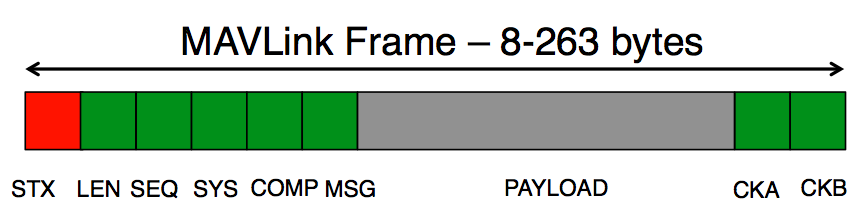
\includegraphics[width=0.5\linewidth]{pics/mavlink}
	\caption{Вращение вокруг оси OZ
	}
	\label{fig:mavlink}
\end{figure}

Первый байт пакета (STX) — это символ начала сообщения: 0xFD для версии v2.0, 0xFE для версии v1.0, 0x55 для версии v0.9. LEN — длинна полезной нагрузки (сообщения). SEQ — содержит счётчик пакета (0-255), который поможет нам выявить потерю сообщения. SYS (System ID) — идентификатор отправляющий системы, а COMP (Component ID) — идентификатор отправляющего компонента. MSG (Message ID) — тип сообщения, от него зависит, какие данные будут лежать в полезной нагрузки пакета. PAYLOAD — полезная нагрузка пакета, сообщение, размером от 0 до 255 байт. Два последних байта пакета — CKA и CKB, нижний и верхний байт, соответственно, содержат контрольную сумму пакета.

Библиотека MAVLink позволяет кодировать и раскодировать пакеты согласно протоколу, но она не регламентирует, какими аппаратными и программными средствами данные будет отправлены — это могут быть TCP/UDP сообщения, обмен через последовательный порт, - все, что обеспечивает двухсторонний обмен. Библиотека обрабатывает входные данные побайтово, добавляя их в буфер и сама собирает из них пакет. Каждая система или компонент, может одновременно обмениваться данными по разным источникам, тогда для каждого источника назначается специальный идентификатор, называемый channel (канал). MAVLink содержит буфер на каждый канал.

\url{https://habr.com/ru/post/312300/}

Канал связи
Протокол MAVLink может быть использован поверх следующих каналов связи:
последовательное соединение (UART, USB и др.);
UDP (Wi-Fi, Ethernet, 3G, LTE);
TCP (Wi-Fi, Ethernet, 3G, LTE).
Сообщение
MAVLink-сообщение это отдельная "порция" данных, передаваемая между устройствами. Отдельное MAVLink-сообщение содержит информацию о состоянии дрона или команду для дрона.

Примеры MAVLink-сообщений:
ATTITUDE, ATTITUDE\_QUATERNION – ориентация квадрокоптера в пространстве;
LOCAL\_POSITION\_NED – локальная позиция квадрокоптера;
GLOBAL\_POSITION\_INT – глобальная позиция квадрокоптера (широта/долгота/высота);
COMMAND\_LONG – команда для квадрокоптера (взлететь, сесть, переключить режим и т. д.).
Полный список MAVLink-сообщений можно посмотреть в документации MAVLink.

Система, компонент системы
Каждое устройство (дрон, базовая станция и т. д.) имеет ID в сети MAVLink. В PX4 MAVLink ID менятся с помощью параметра MAV\_SYS\_ID. Каждое MAVLink сообщение содержит поле с ID системы-отправителя. Кроме того, некоторые сообщения (например, COMMAND\_LONG) содержат также ID системы-получателя.

\url{https://clover.coex.tech/ru/mavlink.html}

\subsection{ROS}

\url{https://www.ros.org/about-ros/}

Robotic Operation System (ROS) - это гибкая платформа для написания программного обеспечения для роботов. Это набор инструментов, библиотек и соглашений, которые призваны упростить задачу создания сложного и надежного поведения роботов на самых разных роботизированных платформах.

Целью создания ROS является создание среды разработки, которая позволяет разработчикам ПО для роботов сотрудничать на глобальном уровне.

ROS сосредоточена на максимизации повторного использования кода при разработке. Основные характеристики позволяющие это реализовать:

Распределенный процессы: Структура ROS создана в виде минимальных единиц исполняемых процессов (нод), и каждый процесс выполняется изолированно. Взаимодействие разных нод происходит только на уровне обмена сообщениями.

Управление пакетами. Несколько процессов, имеющих общую задачу объединяются в пакеты. Управление пакетами подразумевает набор утилит, позволяющие автоматически скачивать, устанавливать и удалять пакеты. Пакетный менеджер гарантирует работоспособность и целостность установленных пакетов.

Публичные репозитории и документация: Каждый доступный пакет публикуется в публичном репозитории. Документация пакетов, публикуется в единой системе, которая упрощает поиск необходимых пакетов.

Единое API: При разработке программы, использующей ROS, вы получаете простое и легко встраиваемое API. В примерах программ вы увидите, что использование API не сильно отличается от языка (C ++ или Python). При этом нет разницы при использовании API на каком языке была написана программа.

Поддержка различных языков программирования: ROS предоставляет клиентские библиотеки для поддержки различных языков программирования. Наиболее популярны Python, C ++, а также такие языки, как Lisp, JAVA, C sharp, Lua и Ruby.

Концепции

Ноды

Основная статья: \url{http://wiki.ros.org/Nodes}

ROS-нода – это специальная программа (обычно написанная на Python или C++), которая взаимодействует с другими нодами посредством ROS-топиков и ROS-сервисов. Разделение сложных робототехнических систем на изолированные ноды дает определенные преимущества: понижается связанность кода, повышается переиспользуемость и надежность.

Очень многие робототехнические библиотеки и драйвера выполнены именно в виде ROS-нод.

Для того, чтобы превратить обычную программу в ROS-ноду, необходимо подключить к ней библиотеку rospy или roscpp и добавить инициализирующий код.

Пример ROS-ноды на языке Python:


\begin{Program}[H]
	\caption{Пример ROS-ноды на языке Python:} \label{lst:1}
	\begin{MyCode}
import rospy

rospy.init_node('my_ros_node')  # имя ROS-ноды

rospy.spin()  # входим в бесконечный цикл...
	\end{MyCode}
\end{Program}
Топики
Основная статья: http://wiki.ros.org/Topics

Топик – это именованная шина данных, по которой ноды обмениваются сообщениями. Любая нода может опубликовать сообщение в произвольный топик, а также подписаться на произвольный топик.

\begin{Program}[H]
	\caption{Пример публикации сообщения типа std\_msgs/String (строка) в топик /foo на языке Python:} \label{lst:1}
	\begin{MyCode}
from std_msgs.msg import String

# ...

foo_pub = rospy.Publisher('/foo', String, queue_size=1)  # создаем Publisher'а

# ...

foo_pub.publish(data='Hello, world!')  # публикуем сообщение
Пример подписки на топик /foo:

def foo_callback(msg):
print msg.data

# Подписываемся. При получении сообщения в топик /foo будет вызвана функция foo_callback.
rospy.Subscriber('/foo', String, foo_callback)
	\end{MyCode}
\end{Program}

Также, существует возможность работы с топиками с помощью утилиты rostopic. Например, с помощью следующей команды можно просматривать сообщения, публикуемые в топик /mavros/state:

rostopic echo /mavros/state

Сервисы

Основная статья: \url{http://wiki.ros.org/Services}

Сервис – это некоторый аналог функции, которая может быть вызвана из одной ноды, а обработана в другой. У сервиса есть имя, аналогичное имени топика, и 2 типа сообщений: тип запроса и тип ответа.

\begin{Program}[H]
	\caption{Пример вызова ROS-сервиса из языка Python:} \label{lst:1}
	\begin{MyCode}
from clover.srv import GetTelemetry

# ...

# Создаем обертку над сервисом get_telemetry пакета clover с типом GetTelemetry:
get_telemetry = rospy.ServiceProxy('get_telemetry', srv.GetTelemetry)

# Вызываем сервис и получаем телеметрию квадрокоптера:
telemetry = get_telemetry()
С сервисами можно также работать при помощи утилиты rosservice. Так можно вызвать сервис /get_telemetry из командной строки:

rosservice call /get_telemetry "{frame_id: ''}"
	\end{MyCode}
\end{Program}

\url{http://docs.voltbro.ru/starting-ros/ros-task.html}

\subsection{MAVROS}
\url{https://clover.coex.tech/ru/mavros.html}
\url{https://dev.px4.io/master/en/ros/mavros_installation.html}

MAVROS (MAVLink + ROS) — это пакет для ROS, предоставляющий возможность управлять беспилотниками по протоколу MAVLink. MAVROS поддерживает полетные стеки PX4 и APM. Связь организовывается по UART, USB, TCP или UDP.

MAVROS подписывается на определенные ROS-топики в ожидании команд, публикует в другие топики телеметрию, и предоставляет сервисы.
Пакет mavros ROS обеспечивает расширяемую связь MAVLink между компьютерами, на которых работает ROS, автопилоты с поддержкой MAVLink и GCS с поддержкой MAVLink.

MAVROS - это «официальный» поддерживаемый мост между ROS и протоколом MAVLink. В настоящее время он расширяется, чтобы включить обмен сообщениями fast-RTPS , включая уровень для преобразования сообщений uORB PX4 в общие идиомы ROS.

Хотя MAVROS может использоваться для связи с любым автопилотом с поддержкой MAVLink, эта документация будет в контексте обеспечения связи между полетным стеком PX4 и компаньоном с поддержкой ROS.
